\chapter{نرم‌افزار}

در این فصل به جزئیات نرم‌افزار پرداخته می‌شود. منظور از نرم‌افزار، کدهایی است که نوشته شده‌اند تا توسط پردازنده‌ی روی ساعت اجرا شوند. در اصطلاح فنی به این بخش سفت‌افزار\footnote{\lr{Firmware}} نیز می‌گویند.

بین سفت‌افزار (برنامه‌ای که روی ریزپردازنده‌ها اجرا می‌شود) و نرم‌افزارهایی که برای سیستم‌های سطح بالا مانند رایانه نوشته می‌شود، تفاوت‌های بسیاری وجود دارد. برای مثال به چند نمونه از این تفاوت‌ها اشاره می‌کنیم:

\begin{enumerate}
	\item عدم وجود سیستم عامل: \\
	برنامه‌هایی که به زبان‌های مختلفی مانند \lr{C} یا \lr{Python} برای رایانه‌ها نوشته می‌شوند، توسط سیستم عامل اجرا می‌شوند. سیستم عامل وظیفه دارد تا برنامه‌های متنوعی که روی سیستم وجود دارد را زمان‌بندی کند، با مدیریت صحیح حافظه آن‌ها را اجرا کند و ارتباط با سخت‌افزار را نیز برعهده بگیرد. اما در حالتی که برای یک ریزپردازنده برنامه می‌نویسیم، دیگر سیستم عاملی وجود ندارد. بلکه تمام برنامه خط به خط و مستقیماً توسط ریزپردازنده اجرا می‌شود.
	
	\item ارتباط مستقیم با سخت‌افزار: \\
	در سیستم‌های سطح بالا که به سیستم عامل مجهزند، ارتباط با سخت‌افزار نیز برعهده‌ی سیستم عامل است. در صورتی که نیاز باشد با دستگاه‌های ورودی/خروجی ارتباطی برقرار شود، از طریق توابع سیستمی موجود در سیستم عامل این ارتباط ایجاد می‌شود. اما هنگام نوشتن برنامه برای ریزپردازنده، باید لایه‌ی ارتباط با سخت‌افزار را نیز نوشت. زیرا سیستم عاملی وجود ندارد و تک تک ارتباطات سخت‌افزاری باید توسط برنامه نویس راه‌اندازی شود.
	
	\item مدیریت حافظه: \\
	هنگامی که در برنامه‌ای به زیان \lr{C} می‌خواهیم از قسمتی از حافظه استفاده کنیم، باید با دستور \lr{malloc} و نظایر آن، به سیستم عامل درخواست دهیم تا آدرس مناسبی را به برنامه‌ی ما اختصاص دهد. همچنین در صورتی که بخواهیم در آدرسی که به برنامه‌ی ما تعلق ندارد مقداری را بنویسیم یا از آن بخوانیم، سیستم عامل مانع می‌شود و با خطای عدم دسترسی مواجه می‌شویم. اما در موردی که با ریزپردازنده‌ها سر و کار داشته باشیم دیگر نیازی به درخواست و اختصاص حافظه نیست. چرا که سیستم عاملی وجود ندارد و تمام حافظه در اختیار برنامه‌ی ما است. در این حالت مدیریت حافظه امری بسیار حساس است. زیرا چیزی وجود ندارد تا مانع دسترسی‌های اشتباه شود و ممکن است با خطا در مدیریت حافظه، عملکرد برنامه دچار اختلالات جدی شود.
	
	\item محدودیت منابع: \\
	پردازنده‌ی رایانه‌ها معمولاً پردازنده‌های قوی‌ای هستند و سرعت بالایی دارند. همچنین حافظه‌های موجود نیز بسیار زیاد هستند. حال آنکه در پردازنده‌ها این منابع بسیار بسیار محدود هستند. همانطور که در ضمیمه‌ی ؟ قابل مشاهده است، مقدار حافظه‌ی فلش ریزپردازنده‌ی ما فقط 64 کیلوبایت است. به این معنی که حجم برنامه بعد از کامپایل نباید از این مقدار تجاوز کند. این محدودیت هرگز در نرم‌افزارهای رایج وجود ندارد. این اتفاق باعث می‌شود تا برنامه نویسی برای ریزپردازنده‌ها دشوارتر شود و نیاز به دانش بیشتری داشته باشد تا بتوان با بهینه‌سازی‌های مختلف و الگوریتم‌های بهتر، حجم برنامه را کاهش داد. در ادامه یکی از این بهینه‌سازی‌ها در رابطه با پیاده‌سازی فیلتر کالمن توضیح داده خواهد شد.
\end{enumerate}

\section{تنظیمات سخت‌افزاری}
همانطور که بالاتر اشاره شد، ارتباط با سخت‌افزار باید توسط برنامه رسیدگی شود. برای این هدف از نرم‌افزار \lr{CubeMX} استفاده شد. شکل \ref{fig:cube-main} نحوه‌ی اختصاص پایه‌ها را نشان می‌دهد. هر کدام از بخش‌ها به تفصیل در ادامه بررسی می‌شود.

	\begin{figure}[h]
		\centering
		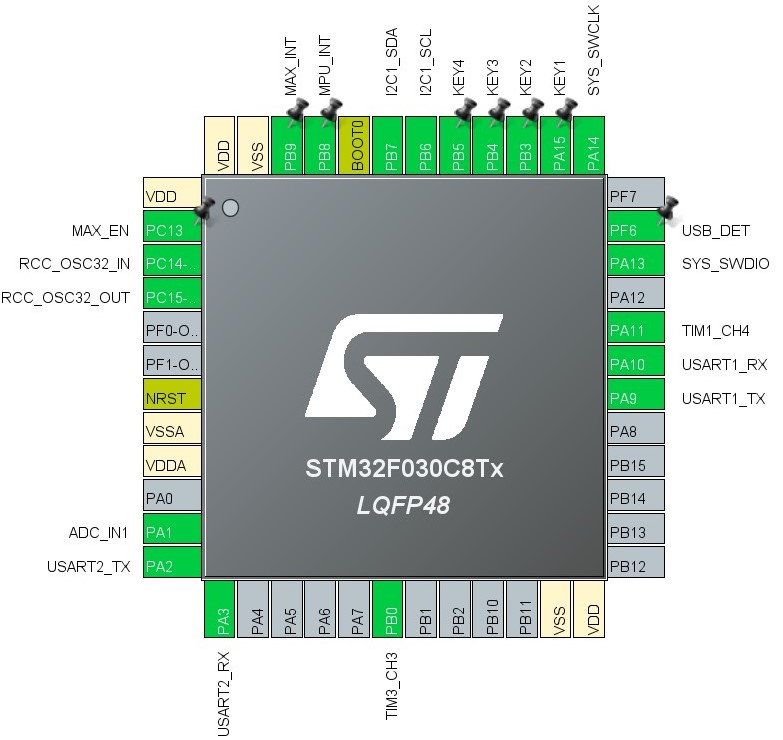
\includegraphics[width=0.9\linewidth]{cube}
		\caption{نحوه‌ی تخصیص پایه‌های مختلف ریزپردازنده در نرم‌افزار \lr{CubeMX}}
		\label{fig:cube-main}
	\end{figure}

\subsection{کلاک}
تنظیمات کلاک به صورت شکل \ref{fig:cube-rcc} است. نوسان‌ساز اصلی روی 8 مگاهرتز داخلی تنظیم شده است و برای ایجاد کلاک بخش ساعت و تاریخ، از یک کریستال خارجی با فرکانس 768.32 کلیوهرتز استفاده شده است. کلاک بخش‌های مختلف نیز در همین تصویر قابل مشاهده است.

	\begin{figure}[h]
		\centering
		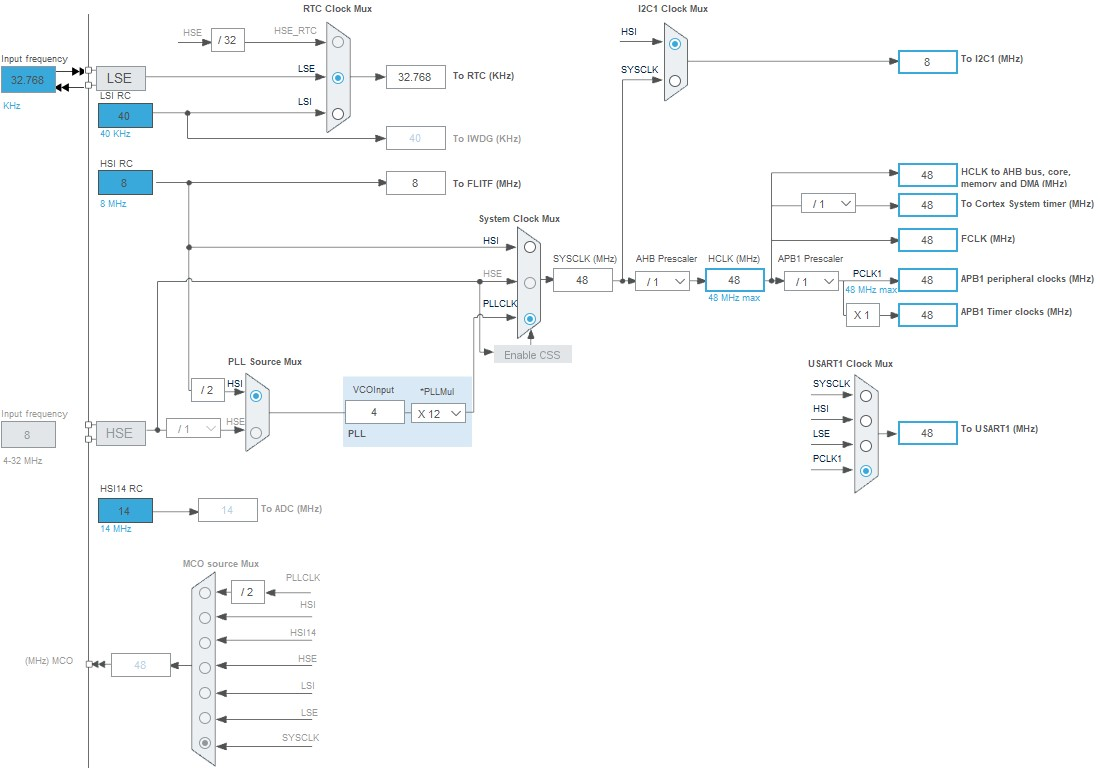
\includegraphics[width=0.9\linewidth]{cube_rcc}
		\caption{تنظیمات کلاک}
		\label{fig:cube-rcc}
	\end{figure}

\subsection{برنامه‌ریزی و اشکال‌زدایی}
برای بحث برنامه‌ریزی\footnote{انتقال برنامه‌ی نوشته شده به ریزپردازنده یا به اصطلاح \lr{Programming}} و اشکال‌زدایی\footnote{\lr{Debugging}} از پروتکل \lr{Serial Wire} استفاده شده است که در شکل \ref{fig:cube-sys} تنظیم آن دیده می‌شود.

	\begin{figure}[h]
		\centering
		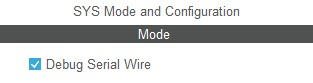
\includegraphics[width=0.4\linewidth]{cube_sys}
		\caption{تنظیمات \lr{Debugging}}
		\label{fig:cube-sys}
	\end{figure}

\subsection{\lr{GPIO}}
\lr{GPIO}ها پایه‌هایی هستند که به عنوان ورودی/خروجی دیجیتال مورد استفاده قرار می‌گیرند. در این پروژه از \lr{GPIO}های متعددی استفاده شده است که در شکل \ref{fig:cube-gpio} فهرست آن‌ها قابل مشاهده است. در ادامه هر مورد توضیح داده می‌‌شود.

	\begin{figure}[h]
		\centering
		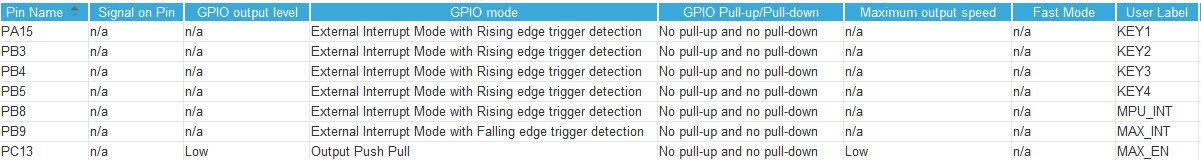
\includegraphics[width=\linewidth]{cube_gpio}
		\caption{تنظیمات \lr{GPIO}}
		\label{fig:cube-gpio}
	\end{figure}

\subsubsection{وقفه‌های خارجی}
وقفه‌های خارجی\footnote{\lr{External intrrupts}}
پایه‌هایی هستند که در صورت وقوع رویداد خاصی، کار عادی پردازنده را متوقف می‌کنند و یک تابع به خصوص را به اجرا در می‌آورند. بعد از اجرای روتین وقفه، پردازنده به کار قبلی خود ادامه می‌دهد.

رویدادهای مورد استفاده در این پروژه دو مورد است: 1- لبه‌ی پایین رونده\footnote{\lr{Falling Edge}}
2- لبه‌ی بالا رونده\footnote{\lr{Rising Edge}}
همانطور که در شکل \ref{fig:cube-gpio} مشهود است، پایه‌های 3، 4، 5 و 8 از پورت \lr{B} و پایه‌ی 15 از پورت \lr{A} برای لبه‌ی بالارونده تنظیم شده‌اند. پایه‌ی 9 از پورت \lr{B} نیز به لبه‌ی پایین رونده حساس است.

اینکه کدام پایه توسط کدام بخش تحریک می‌شود در ستون \lr{User label} شکل \ref{fig:cube-gpio} دیده می‌شود. برچسب‌های \lr{KEY} مربوطه به کلیدهای لمسی روی بدنه هستند. در صورت لمس شدن هر کلید، تابع مخصوص آن اجرا می‌شود. برچسب \lr{MPU} مربوط به حسگر حرکتی است. این پایه وقتی فعال می‌شود که داده‌های جدید حسگر آماده شده باشد. برچسب \lr{MAX} نیز به همین شکل عمل می‌کند. هرگاه داده‌ی حسگر \lr{PPG} آماده‌ی قرائت باشد، این وقفه فعال می‌شود.

\subsubsection{خروجی دیجیتال}
پایه‌ی 13 از پورت \lr{C} به صورت خروجی دیجیتال تعریف شده است. این خروجی به پایه‌ی فعالساز سوییچ ماسفتی متصل است که حسگر \lr{PPG} را روشن می‌کند (شکل \ref{fig:sch-ppg}). برای روشن یا خاموش کردن این حسگر، کافی است این پایه را صفر یا یک کرد.

\subsection{\lr{RTC}}
واحد
\lr{RTC}\footnote{\lr{Real-time Clock}}
برای نگهداری و کار با ساعت و تاریخ است. تنظیمات این بخش در شکل \ref{fig:cube-rtc} دیده می‌شود. در این بخش می‌توان یک آلارم هم فعال کرد که در ساعت و روز مشخصی یک وقفه را فعال کند. در اینجا آلارم هم فعال شده است.

	\begin{figure}[h]
		\centering
		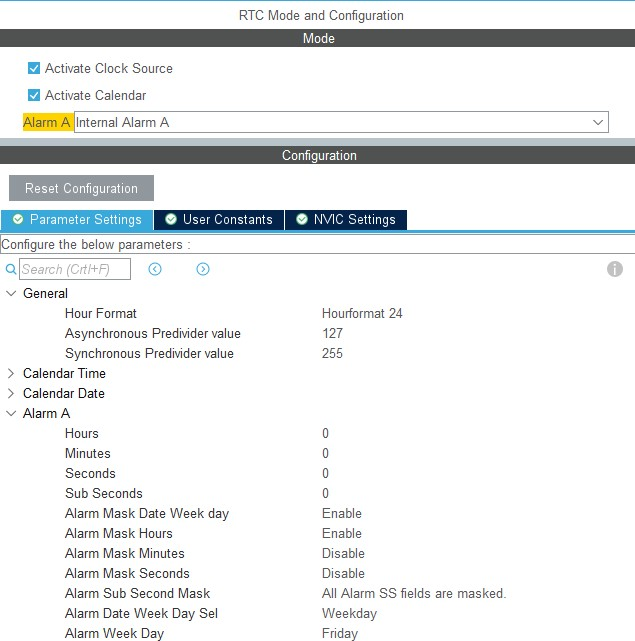
\includegraphics[width=0.45\linewidth]{cube_rtc}
		\caption{تنظیمات \lr{RTC}}
		\label{fig:cube-rtc}
	\end{figure}

\subsection{تایمرها}
این ریزپردازنده هفت تایمر دارد که در این پروژه هر هفت تایمر استفاده شده‌اند. در ادامه کاربرد و تنظیمات هر تایمر شرح داده می‌شود.

\subsubsection{\lr{TIM1}}
تایمر شماره‌ی یک مطابق با تنظیمات شکل \ref{fig:cube-tim1} راه‌اندازی شده است تا بتواند \lr{PWM} موردنیاز برای کنترل دور موتور ایجاد لرزش را تولید کند. البته مقدار رجیستر \lr{ARR} در برنامه به صورت پویا تغییر می‌کند.

\subsubsection{\lr{TIM3}}
تایمر شماره‌ی یک مطابق با تنظیمات شکل \ref{fig:cube-tim3} راه‌اندازی شده است تا بتواند \lr{PWM} موردنیاز برای تنظیم فرکانس صدای بازر را تولید کند. البته مقدار رجیستر \lr{ARR} در برنامه به صورت پویا تغییر می‌کند.

	\begin{figure}[h]
		\centering
		\begin{subfigure}{0.4\textwidth}
			\centering
			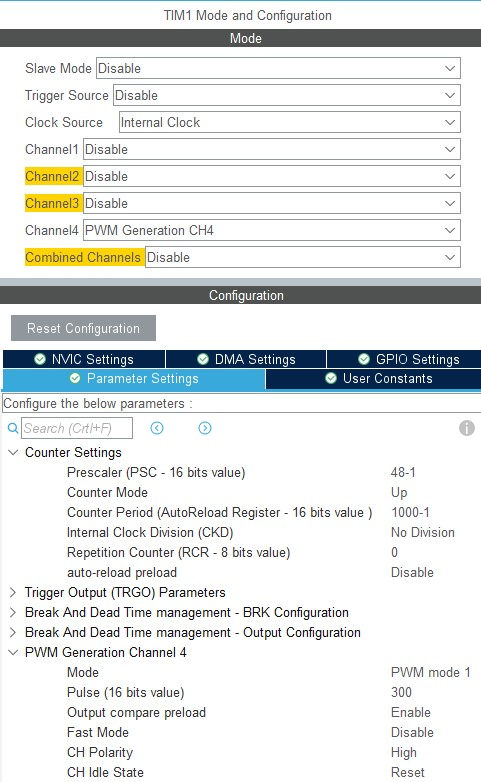
\includegraphics[width=\linewidth]{cube_tim1}
			\caption{تنظیمات تایمر یک}
			\label{fig:cube-tim1}
		\end{subfigure}
		\begin{subfigure}{0.44\textwidth}
			\centering
			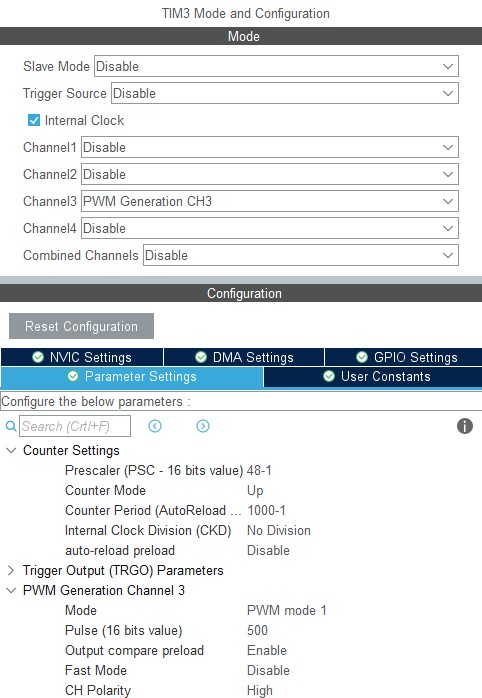
\includegraphics[width=\linewidth]{cube_tim3}
			\caption{تنظیمات تایمر سه}
			\label{fig:cube-tim3}
		\end{subfigure}
		\caption{تنظیمات دو تایمر}
		%\label{fig:body-pcb}
	\end{figure}

\subsubsection{\lr{TIM6}}
تایمر شماره‌ی شش مطابق شکل \ref{fig:cube-tim6} تنظیم شده است تا هر یک میلی ثانیه یک وقفه را فعال کند. این وقفه توابع مربوط به فیلتر کالمن را اجرا می‌کند. در واقع می‌توان گفت دوره تناوب نمونه‌گیری و پردازش سیستم کالمن یک میلی ثانیه است.

	\begin{figure}[h]
		\centering
		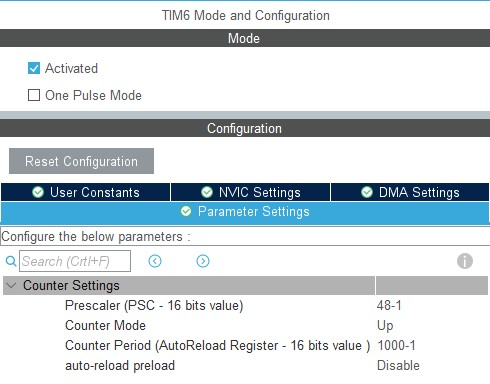
\includegraphics[width=0.43\linewidth]{cube_tim6}
		\caption{تنظیمات تایمر شش}
		\label{fig:cube-tim6}
	\end{figure}

\subsubsection{\lr{TIM14}}
تایمر شماره‌ی چهارده مطابق شکل \ref{fig:cube-tim14} تنظیم شده است تا هر 250 میلی ثانیه یک وقفه را فعال کند. این وقفه مربوط به توابع سیستمی است. در این توابع مواردی از قبیل تازه‌سازی صفحه نمایش و تنظیم برخی متغیرها انجام می‌شود.


	\begin{figure}[h]
		\centering
		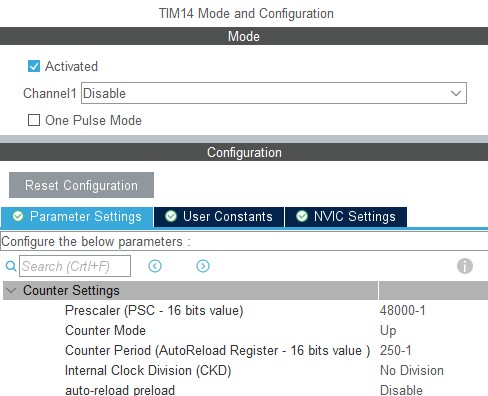
\includegraphics[width=0.35\linewidth]{cube_tim14}
		\caption{تنظیمات تایمر چهارده}
		\label{fig:cube-tim14}
	\end{figure}

\subsubsection{\lr{TIM15}}
تایمر شماره‌ی پانزده مطابق شکل \ref{fig:cube-tim15} تنظیم شده است تا هر 10 میلی ثانیه به واحد \lr{ADC} فرمانِ تبدیل دهد. به این معنی که واحد آنالوگ به دیجیتال فقط در صورتی یک نمونه‌برداری را شروع می‌کند که تایمر شماره 15 به آن فرمان دهد. اینگونه یک نمونه‌برداری دقیق زمانی ایجاد می‌شود.

	\begin{figure}[h]
		\centering
		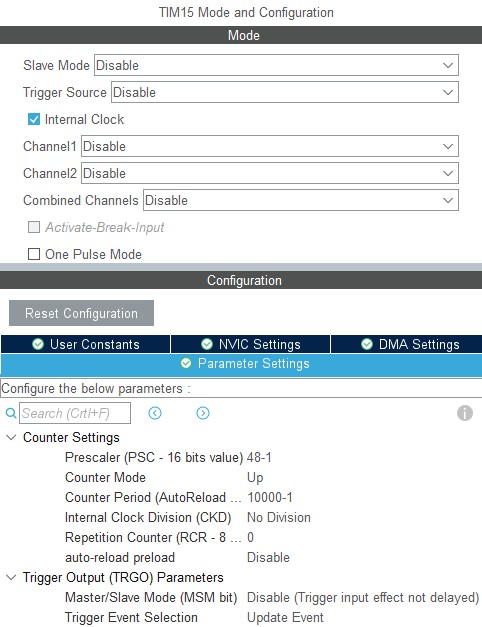
\includegraphics[width=0.4\linewidth]{cube_tim15}
		\caption{تنظیمات تایمر پانزده}
		\label{fig:cube-tim15}
	\end{figure}

\subsubsection{\lr{TIM16}}
تایمر شماره‌ی شانزده مطابق شکل \ref{fig:cube-tim16} تنظیم شده است تا هر 4 ثانیه یک وقفه را فعال کند. این وقفه برای خاموش کردن صفحه نمایش است. هرگاه کاربر به مدت 4 ثانیه با ساعت تعامل نداشته باشد این وقفه صفحه را خاموش می‌کند.

	\begin{figure}[h]
		\centering
		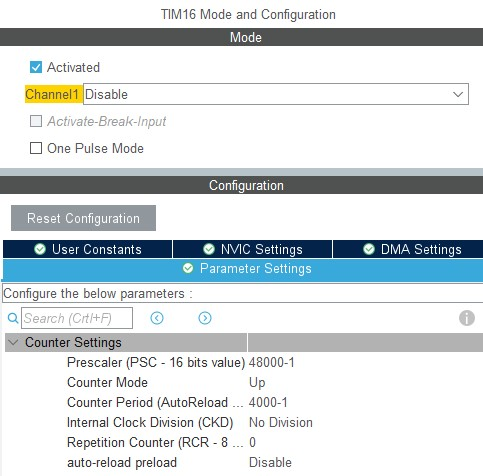
\includegraphics[width=0.4\linewidth]{cube_tim16}
		\caption{تنظیمات تایمر شانزده}
		\label{fig:cube-tim16}
	\end{figure}

\subsubsection{\lr{TIM17}}
تایمر شماره‌ی هفده مطابق شکل \ref{fig:cube-tim17} تنظیم شده است. این تایمر وقفه ندارد و به صورت یک زمان‌سنج به کار می‌رود. از این تایمر برای ساخت تابع تأخیر استفاده شده است. حداکثر تأخیر قابل تولید توسط این تایمر، دو به توان 16 یعنی 65536 میلی ‌ثانیه است. 

	\begin{figure}[h]
		\centering
		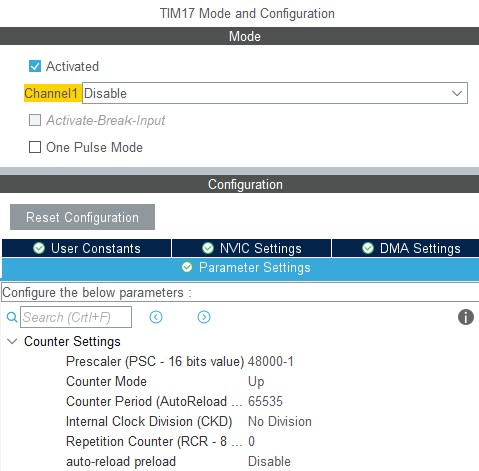
\includegraphics[width=0.4\linewidth]{cube_tim17}
		\caption{تنظیمات تایمر هفده}
		\label{fig:cube-tim17}
	\end{figure}

\subsection{\lr{ADC}}
مبدل آنالوگ به دیجیتال در این پردازنده 12 بیتی است. یعنی ولتاژ ورودی را از بازه‌ی 0 تا 3.3 ولت به بازه‌ی 0 تا 4095 نگاشت می‌کند. اینگونه می‌توان با یک ضرب و تقسیم ساده مقدار ولتاژ ورودی را خواند. شکل \ref{fig:cube-adc} تنظیمات این واحد را نشان می‌دهد. همانطور که گفته شد، این واحد به کمک تایمر 15 فعال می‌شود و با هر فرمان آن یک نمونه برمی‌دارد. برای ذخیره‌ی این نمونه‌ها، \lr{ADC} را با
\lr{DMA}\footnote{\lr{Direct Memory Access}}
کوپل می‌کنیم. اینگونه هربار که \lr{ADC} یک نمونه را تبدیل کرد، به طور مستقیم و بدون دخالت پردازنده آن را در یک آرایه ذخیره می‌کند. بعد از اینکه آرایه پر شد نیز با فعال کردن یک وقفه به ما خبر می‌دهد تا عملیات پردازشی روی آن انجام گیرد.

این ساختار که \lr{ADC} با تایمر فعال شود و با \lr{DMA} کار کند، حرفه‌ای ترین ساختار راه‌اندازی این واحد است. تنظیمات \lr{DMA} در شکل \ref{fig:cube-adc-dma} دیده می‌شود.

	\begin{figure}[h]
		\centering
		\begin{subfigure}{0.5\textwidth}
			\centering
			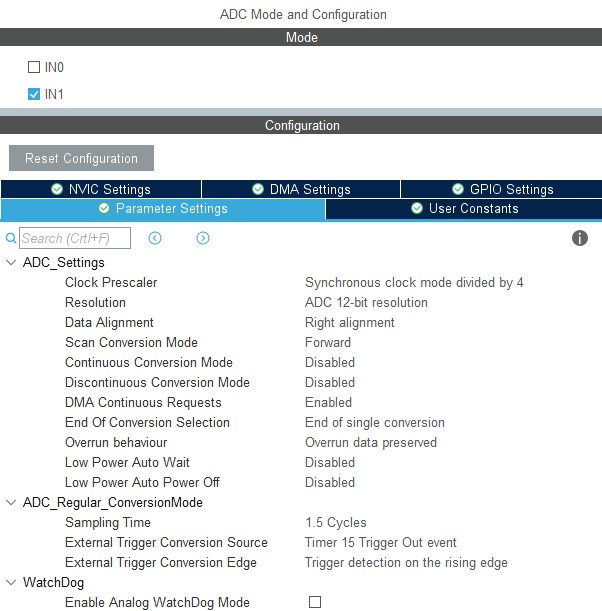
\includegraphics[width=\linewidth]{cube_adc}
			\caption{تنظیمات \lr{ADC}}
			\label{fig:cube-adc}
		\end{subfigure} \\
		\begin{subfigure}{0.54\textwidth}
			\centering
			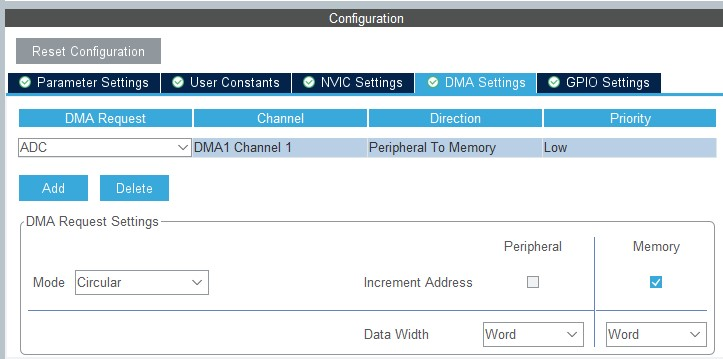
\includegraphics[width=\linewidth]{cube_adc_dma}
			\caption{تنظیمات \lr{DMA}}
			\label{fig:cube-adc-dma}
		\end{subfigure}
		\caption{تنظیمات مبدل آنالوگ به دیجیتال}
	\end{figure}

\subsection{\lr{I2C}}
واحد \lr{I2C} مطابق شکل \ref{fig:cube-i2c} تنظیم شده است. این واحد یک واحد ارتباطی تحت پروتکل \lr{I2C} است.

	\begin{figure}[h]
		\centering
		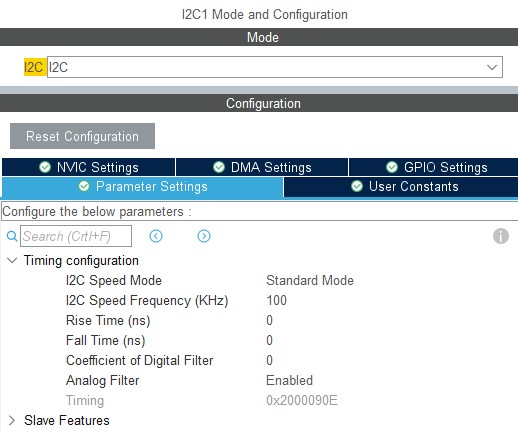
\includegraphics[width=0.5\linewidth]{cube_i2c}
		\caption{تنظیمات \lr{I2C}}
		\label{fig:cube-i2c}
	\end{figure}

\subsection{\lr{USART}}
واحد \lr{USART1} و \lr{USART2} مطابق شکل \ref{fig:cube-usart} تنظیم شده و تنظیمات مشابهی دارند. با این تفاوت که \lr{USART2} به یک واحد \lr{DMA} نیز وصل است تا داده‌ی دریافتی بلوتوث را مستقیماً در حافظه ذخیره کند و در صورت تکمیل شدن پیام، وقفه‌ی مربوطه را فعال کند تا داده‌ی دریافتی پردازش شود.

	\begin{figure}[h]
		\centering
		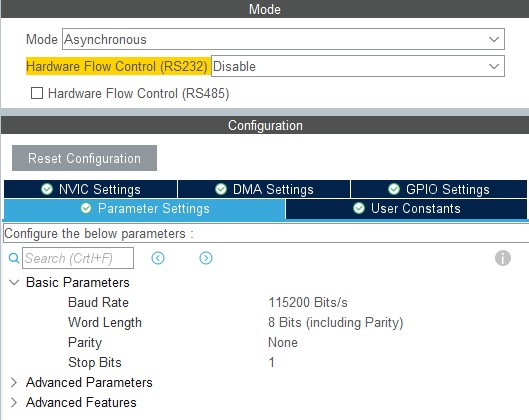
\includegraphics[width=0.5\linewidth]{cube_usart}
		\caption{تنظیمات \lr{USART}}
		\label{fig:cube-usart}
	\end{figure}

\section{معماری}
آره خلاصه